\begin{frame}
    \begin{definition}
        Elementar $\colon\!\!\Leftrightarrow$ Beträge meromorpher Funktionen bilden eine Garbe, 
        d.h. aus $|f_i| = |f_j|$ auf $U_i \cap U_j \forall i, j \in I$ folgt die Existenz einer meromorphen Funktion $f \colon X \to \C$ mit $|f| = |f_i|$ auf $U_i$.
    \end{definition}
    \begin{theorem}[Monodromiesatz]
        Sei $X$ eine einfach zusammenhängende Riemann'sche Fläche und $f \colon U(a) \to \overline{\C}$ entlang jedes von $a$ ausgehenden Weges fortsetzbar. Dann existiert eine meromorphe Funktion $F\colon X \to \overline{\C}$ mit $F|_{U(a)} = f$.
    \end{theorem}
    \begin{lemma}
        Einfach zusammenhängende Riemannsche Flächen sind elementar.
    \end{lemma}
    
\end{frame}
\begin{frame}
    \begin{lemma}
        Einfach zusammenhängende Riemannsche Flächen sind elementar.
    \end{lemma}
    \begin{proof}
        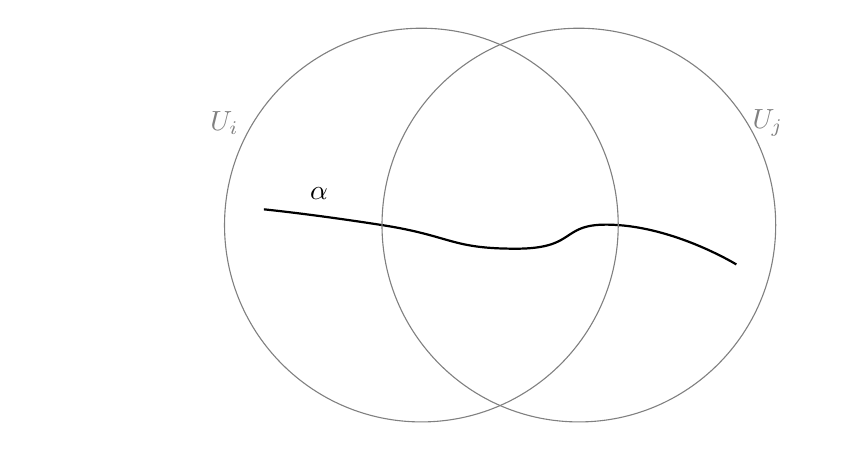
\begin{tikzpicture}
            \path (-5,0) -- (5,0);
            \draw [black,thick] plot [smooth,samples=200, tension=1] coordinates { 
                (-2,0.2) (-.5,0) (1.2,-.3) (2.5,0) (4,-.5)};
            %\draw [blue,thick] plot [smooth,samples=200, tension=1] coordinates { 
            %    (-.5,.1) (1.2,-.2) (2.5,.1) (4,-.4)};
            %\draw [red,thick] plot [smooth,samples=200, tension=1] coordinates { 
            %    (-2,0.1) (-.5,-.1) (1.2,-.4) (2.2, -.1) (2.5,-.1)};
            \draw[gray] (0,0) circle (2.5);
            \draw[gray] (2,0) circle (2.5);
            \node[black] (alpha) at (-1.3,.4) {$\alpha$};
            %\node[red] (fi) at (-2,-.2) {$f_i$};
            %\node[blue] (fj) at (4,-.1) {$f_j$};
            \node[gray] (Ui) at (-2.5,1.3) {$U_i$};
            \node[gray] (Uj) at (4.4,1.3) {$U_j$};
          \end{tikzpicture}
    \end{proof}
\end{frame}
\begin{frame}
    \begin{lemma}
        Einfach zusammenhängende Riemannsche Flächen sind elementar.
    \end{lemma}
    \begin{proof}
        \begin{itemize}
            \item $|f_i/f_j| = 1$ auf $U_i \cap U_j \implies f_i/f_j = c_{ij}$
            \item Setze $f_i$ fort durch $c_{ij} \cdot f_j$
            \item Erhalte $f$ mit $f/f_k = \mathrm{const}$ auf $U_k$ mit $|f/f_k| = 1$. 
        \end{itemize}
    \end{proof}
\end{frame}

%\begin{proof}
    %    Sei $X = \bigcup U_i$ eine offene Überdeckung von $X$ und sei $f_i\colon U_i \to \overline{\C}$ eine Schar 
    %    invertierbarer (\textbf{Warum?}) meromorpher Funktionen mit der Eigenschaft $|f_i/f_j| = 1$ auf $U_i \cap U_j$.
    %    Man kann nun für ein $a \in U_i$ analytische Fortsetzungen für $f_i$ entlang von Wegen auf $U_i$ konstruieren, indem man auf $U_j$ die Funktion $f_j$ benutzt und diese mit dem konstanten (Maximumprinzip) Faktor $c_{ij} = |f_i/f_j|$ multipliziert. So kann man $f_i$ auf $U_j$ analytisch fortsetzen.
    %    Da $X$ einfach zusammenhängend ist, erhält man nach dem Monodromiesatz eine meromorphe Fortsetzungen von $f_i$ auf ganz $X$. Nach Konstruktion ist auf $U_k$ dann $f/f_k$ konstant und vom Betrag 1.
    %\end{proof}